\section{Muster}

\subsection{Entwurfsmuster}

\begin{defi}{Entwurfsmuster}
    Entwurfsmuster sind bewährte Lösungsschablonen für wiederkehrende Entwurfsprobleme sowohl in der Architektur als auch in der Softwarearchitektur und -entwicklung.

    Sie stellen damit eine wiederverwendbare Vorlage zur Problemlösung dar, die in einem bestimmten Zusammenhang einsetzbar ist.

    Es gibt verschiedene Typen von Entwurfsmustern.
    Es werden folgende Typen unterschieden:
    \begin{itemize}
        \item \emph{Erzeugungsmuster (Creational Patterns)}:
              Dienen der Erzeugung von Objekten. Sie entkoppeln die Konstruktion eines Objekts von seiner Repräsentation.
              \begin{itemize}
                  \item Fabrikmethode (Factory method)
                  \item Abstrakte Fabrik (Abstract Factory)
                  \item Erbauer (Builder)
                  \item Prototyp (Prototype)
                  \item Singleton
              \end{itemize}
        \item \emph{Strukturmuster (Structural Patterns)}:
              Erleichtern den Entwurf von Software durch vorgefertigte Schablonen für Beziehungen zwischen Klassen.
              \begin{itemize}
                  \item Schablonenmethode (Template method)
                  \item Beobachter (Observer)
                  \item Iterator
                  \item Besucher (Visitor)
                  \item Strategie (Strategy)
                  \item Zustand (State)
              \end{itemize}
        \item \emph{Verhaltensmuster (Behavioral Patterns)}:
              Modellieren komplexes Verhalten der Software und erhöhen damit die Flexibilität der Software hinsichtlich ihres Verhaltens.
              \begin{itemize}
                  \item Stellvertreter (Proxy)
                  \item Kompositum (Composite)
                  \item Fassade (Facade)
                  \item Dekorierer (Decorator)
              \end{itemize}
    \end{itemize}
\end{defi}

\begin{defi}{Strategie-Muster}
    Das Strategie- (Strategy) Muster ist im Bereich der Softwareentwicklung ein Entwurfsmuster und gehört zur Kategorie der Verhaltensmuster.

    Eine Strategie definiert eine Familie (zur Laufzeit) austauschbarer Algorithmen.

    \begin{center}
        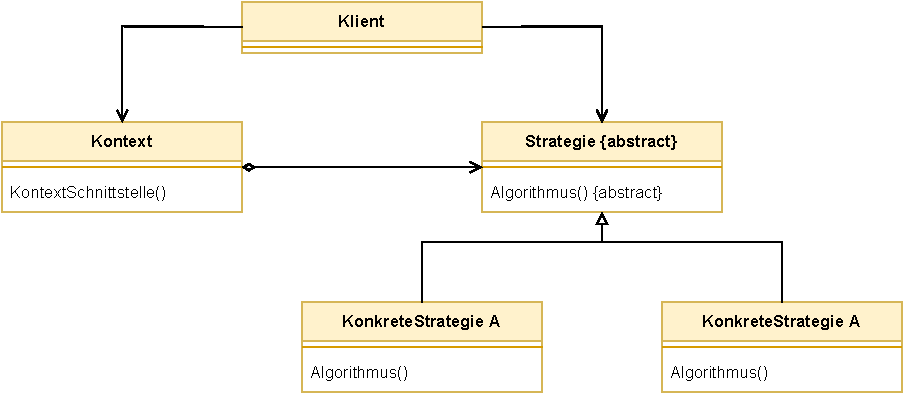
\includegraphics[width=0.7\textwidth]{includes/figures/defi_strategie.pdf}
    \end{center}
\end{defi}

\begin{example}{Strategie-Muster}
    % Wir definieren zuerst das Strategie-Interface \texttt{CatchStrategy} und zwei Implementierungen \texttt{PokeBallCatchStrategy} und \texttt{MasterBallStrategy}:
    \lstinputlisting[language=java]{includes/code/CatchStrategy.java}

    % Dann definieren wir einen Klienten, der eine beliebige Strategie verwendet:
    \lstinputlisting[language=java]{includes/code/Ball.java}

    % Die Verwendung sieht dann z.B. so aus:
    \lstinputlisting[language=java]{includes/code/StrategyExample.java}
\end{example}


\begin{defi}{Beobachter-Muster}
    Das Beobachter- (Observer) Muster ist im Bereich der Softwareentwicklung ein Entwurfsmuster und gehört zur Kategorie der Verhaltensmuster.

    Ein Beobachter dient der Weitergabe von Änderungen an einem Objekt an von diesem Objekt abhängige Strukturen.

    \begin{center}
        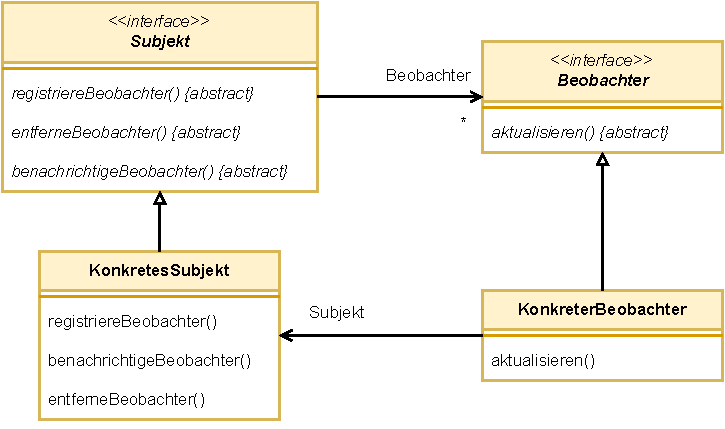
\includegraphics[width=0.7\textwidth]{includes/figures/defi_beobachter.pdf}
    \end{center}
\end{defi}

\begin{example}{Beobachter-Muster}
    % Zuerst definieren wir die Klasse \texttt{BattleNews} und die Klasse \texttt{Trainer} als Beobachter:
    \lstinputlisting[language=java]{includes/code/BattleNews.java}

    % Danach definieren wir die \texttt{NewsChannel} Klasse, die abonniert werden soll:
    \lstinputlisting[language=java]{includes/code/NewsChannel.java}

    % Die Verwendung sieht dann z.B. so aus:
    \lstinputlisting[language=java]{includes/code/BeobachterExample.java}
\end{example}

\begin{defi}{Singleton-Muster}

\end{defi}

\begin{example}{Singleton-Muster}

\end{example}

\begin{defi}{Fabrikmethode}

\end{defi}

\begin{example}{Fabrikmethode}

\end{example}

\begin{defi}{Fassade-Muster}

\end{defi}

\begin{example}{Fassade-Muster}

\end{example}

\begin{defi}{Dekorierer-Muster}

\end{defi}

\begin{example}{Dekorierer-Muster}

\end{example}

\begin{defi}{Kompositum-Muster}

\end{defi}

\begin{example}{Kompositum-Muster}

\end{example}

\begin{defi}{Singleton-Muster}

\end{defi}

\begin{example}{Singleton-Muster}

\end{example}

\begin{defi}{Zustand-Muster}

\end{defi}

\begin{example}{Zustand-Muster}

\end{example}

\begin{defi}{Kohäsion}

\end{defi}

\begin{defi}{Kopplung}

\end{defi}

\subsection{Architekturmuster}

\begin{defi}{Architekturmuster}

\end{defi}

\begin{defi}{Schichten-Muster}

\end{defi}

\begin{defi}{Pipes und Filter}

\end{defi}

\begin{defi}{Model-View-Controller}

\end{defi}

\begin{defi}{Client-Server}

\end{defi}